%----------------------------------------------------------------------------------------
%	PACKAGES AND DOCUMENT CONFIGURATIONS
%----------------------------------------------------------------------------------------

\documentclass{article}

\usepackage[version=3]{mhchem} % Package for chemical equation typesetting
\usepackage{siunitx} % Provides the \SI{}{} and \si{} command for typesetting SI units
\usepackage{graphicx} % Required for the inclusion of images
\usepackage{natbib} % Required to change bibliography style to APA
\usepackage{amsmath} % Required for some math elements 
\usepackage{enumitem}% For lists
\usepackage{mathptmx}% For textbf
\usepackage{float} %for correct image placement
\usepackage{textcomp} % for texttildelow
\usepackage[T1]{fontenc} % allows use of less than <
\usepackage{booktabs} % for tables


\setlength\parindent{0pt} % Removes all indentation from paragraphs

\renewcommand{\labelenumi}{\alph{enumi}.} % Make numbering in the enumerate environment by letter rather than number (e.g. section 6)

%\usepackage{times} % Uncomment to use the Times New Roman font

%----------------------------------------------------------------------------------------
%	DOCUMENT INFORMATION
%----------------------------------------------------------------------------------------

\title{M152A - Lab 4 \\ Design Lab \\ The Multiplayer Tank Experience} % Title

\author{Markus \textsc{Notti} - 904269231 \\ Kyle \textsc{Baker}  - 604273748 \\ Niels \textsc{Pineda} - 604272353} % Author name


\date{\today} % Date for the report

\begin{document}

\maketitle % Insert the title, author and date

%----------------------------------------------------------------------------------------
%	SECTION 1
%----------------------------------------------------------------------------------------

\section*{Introduction}

%Summarize background information
%about the lab and the detailed design requirements. It?s very important to
%make sure you are designing the right thing before starting.

In this lab, we implemented a basic multiplayer tank game utilizing the VGA for the main display, buttons and switches on the board for controls, and the seven segment display for additional in game information display.

Our game was played in the following manner:
Each of the two players playing the game controls a tank and fires projectiles at his opponent from the opposite side of the map, displayed on the VGA.  To fire, the player 1 and player 2 would press the \textit{fire1} and \textit{fire2} buttons respectively. As the players fire the projectiles using the buttons on the FPGA board, the players are also able to adjust the initial velocity and angle of the projectiles using additional buttons.  How long the \textit{fire1} and \textit{fire2} buttons are held down by the players determines the projectiles' initial velocity, and the angle can be adjusted by clicking either the \textit{angleUp} button to raise the angle or the \textit{angleDown} button to lower the angle. 
\\
\\
If a player's tank is struck by a hostile projectile, the player's tank loses health, which is immediately updated on the 7-segment display. If the projectile makes a direct hit upon the tank, the player's health is reduced by 14HP. If it is only a glancing blow the player's health is reduced by only 7HP.  The health display for both of the players' healths was also configured to display the player's own health facing the correct player. In other words, since the players themselves must be on opposite sides of the board to play the game, each player can see his own health, because it is flipped to the perspective of the player who's health it is displaying. 

If a tank reaches a health of 0HP, that tank turns red marking the end of the game and victory for the player controlling the other tank.  The game can then be reset by flipping the \textit{rst} switch on the board.
\\
\\
Behind the scenes, a clock module, which along with the other modules, will be discussed in more detail later, created three separate clocks which would drive the program.  The three clocks created were 25MHz, 500Hz, and 50Hz.  The 25MHz clock was responsible for driving the VGA controller, the 500Hz clock drove the seven segment display, and the 50Hz clock was responsible for updating the position of the tanks and the projectiles on screen. 
\\

In order for all of this gameplay to be a reality, we needed to design and implement the following set of features:
%TODO: pdf/screenshot of the features list (as edited by matt millar himself)
 
%----------------------------------------------------------------------------------------
%	SECTION 2
%----------------------------------------------------------------------------------------

\section*{Design Description}

%Design description (15%). Document the design aspects including the basic
%description of the design, modular architecture, interactions among the
%modules, and interface of each major module. You should include schematics
%for the system architecture. You can also include figures for state machines
%and Verilog code when needed.

% TODO: Make circuit diagram
% TODO: Make sure the figures referenced are correct

When designing the lab, we created 8 main modules \textit{clock}, \textit{vga}, \textit{sevenSeg}, \textit{tankL}, \textit{tankR}, \textit{projL}, \textit{projR} and \textit{collisionDetector} all running in the main module \textit{game}.  The clock module created 3 slower clocks to regulate other parts of the program, while the rest of the modules, their names relatively self explanatory, contained the program's logic.

\subsection*{Clock Module - \textit{clock}}

The clock module took as input a 100MHz clock and outputted three separate clocks to govern the rest of the program: a 25MHz clock, a 500Hz clock, and a 50Hz clock.  This was implemented by 3 simple counters. The 25MHz counter would count to 4, the 500Hz clock would count to 200,000, and the 50Hz clock would run to 2,000,000.  At the posedge of the 100MHz clock, the counts would increment until they reached their respective maximums, triggering the appropriate output clocks to 1. After reaching this maximum value, the counters would drop back to zero and start their counts over again.  This clock module was the beating heart of our software, controlling the rates at which all logic would be calculated, all input would be read and all output would be written.

\subsection*{VGA Module - \textit{vga}}

Our VGA module was essentially a controller we designed to handle the VGA functionality for the program.  This was probably the most complicated of the lab for us, because it took a lot of trial and error to get it working.  Our VGA controller module takes as the 25MHz clock created by the clock module and produces as output 8 wires which make up the color composition of the pixel to be drawn and two wires \textit{Hsync} and \textit{Vsync} to govern the VGA.  \\
\\
In order to implement this controller, two counters, \textit{counterX} and \textit{counterY}, tracked the location of the VGA sweep as it swept across the screen and down the screen.  In addition to tracking the location of the VGA sweep on the 640x480 display to figure out when to draw what pixels, the counters were responsible for tracking when exactly it was even appropriate to begin outputting values to the 8 wires governing the pixel color. The tricky part about designing the VGA controller was this specific timing.  As illustrated further by the image below, there are very specific periods of time where no color combination must be output, and there are specific times when the \textit{Hsync} and \textit{Vsync} must be fired to indicate that a new section of the display is about to be drawn.  For every line, there would be a front porch for 8 cycles, a horizontal sync period where Hsync would be fired for 96 cycles, a back porch for 40 cycles, an 8 cycle left border, then a 480 cycle display followed by an 8 cycle right border.  For the periods mentioned above, the colors outputted by the vga module to the VGA were all set to 0.  \textit{counterX} tracked how many cycles had passed to give the program working knowledge of what period it was in. During the display period is where the appropriate objects were drawn to screen.  The Vertical Sync had similar periods with slightly different cycle count.  The exact count is displayed below in the image.  Note that where the image says 'pixels', we implemented our controller so that each cycle moved onto the next pixel, so in this situation, pixels can be considered equivalent to cycles.

\begin{figure}[H]
	\begin{center}
		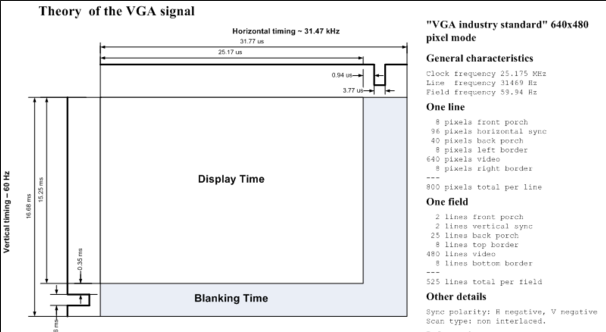
\includegraphics[width=1\textwidth]{vgaTheory} 
		\caption{Basic VGA theory upon which we based our VGA controller}
	\end{center}
\end{figure}

\subsection*{Seven Segment Display Module - \textit{sevenSeg}}

This module was the controller we designed to handle the seven segment display.  It would be passed both of the players' healths and it would display player 1's health facing him, and player 2's health facing opposite, so each of the players can look down at the seven segment display from his respective side of the board and see how much health he has remaining. \\
\\
The encoding of the tank health into a form readable and displayable by the seven segment display was done using two priority encoders, one for the digits that faced player 1, and one for the digits that faced player 2.  Once the digits were all encoded by the priority encoders, the 4 digits were  separately displayed at a frequency of 500Hz, governed by a clock that was passed into the module as input after being created by the clock module.  By displaying only one digit at a time, and displaying a different digit 500 times a second, it seems to the human eye that all four digits are being displayed simultaneously.

\subsection*{Tank Module - \textit{tankL}, \textit{tankR}}

The tank module was designed with the purpose of controlling the location and the movement of both players' tanks on screen.  While it didn't make them actively move across the screen, the job of the VGA controller, the tank module looked for movement button presses from the players and updated the tanks' positions accordingly, outputting them to the projectile modules so they knew where to place the projectiles on screen upon initially firing, and to the VGA module so that the VGA knew where to draw them.  
\\
\\
Not only did the tank module handle listening for movement buttons \textit{btnL} and \textit{btnR} in order to update the position of the tanks accordingly, it also listened for \textit{angleUp} and \textit{angleDown} buttons to adjust the angles at which the projectiles would be firing from the tanks.  Every time either the angle up or angle down buttons would be pressed, the tank module would add or subtract 5 degrees from the angle of the relevant tank.  This angle value would then be passed into the projectile module.
\\
\\
It should also be noted that due to some minor issues we had when we created two instances of the tank module, one for player 1 and one for player 2, we decided to do a quick work around and make them two separate modules.  Since they are effectively the same, I have considered them the same for the sake of this report.

\subsection*{Projectile Module - \textit{projL}, \textit{projR}}

The projectile module contained all of the logic required to simulate the motion of the projectile as if its been fired from the barrel of a cannon.  This module takes as input the tank's location and the angle at which that tank is currently set to fire its projectile.  The projectile module then takes the angle and uses a priority encoder to retrieve the correct initial x and y velocities at which it should be fired.  Then, if the appropriate fired button is pressed, the projectile takes the initial position of the appropriate tank and is assigned the initial velocities found by the priority encoder.  Next, the new position of the projectile is determined 50 times a second, and is outputted to vga to be displayed.  In order to keep the projectiles flight from being adversely affected by the movement of the tank while the projectile is in flight, updates to the tank's initial position and angle are stopped while the projectile is in flight. Once the projectile hits its target or falls off the screen, the projectile module begins again to listen.
\\
\\
Like the tank module mentioned above, the same problem was occurring for us, so we went ahead and made two separate projectile modules, as it solved our problem.  However, in the same way, I have considered them two instances of the same module for the sake of simplicity in explanation.

\subsection*{Collision Detector Module - \textit{collisionDetector} }

The collision detector module, as the name suggests, was responsible for monitoring the positions of the tank modules and the projectile modules and listening for any overlap.  It was also responsible for relaying that information to the rest of the program. It simply would take in as input all of the positions of the objects mentioned above and check for overlap.  If there was overlap, it would simply set a t1\_col flag to 1 or a t2\_col flag to 1 depending on which tank was hit.  The projectile module would pick up this flag and reset, and the seven segment controller module would also pick up this flag and update the health of the tanks on the display accordingly.

\subsection*{Digital Logic Design}
\begin{figure}[H]
	\begin{center}
		%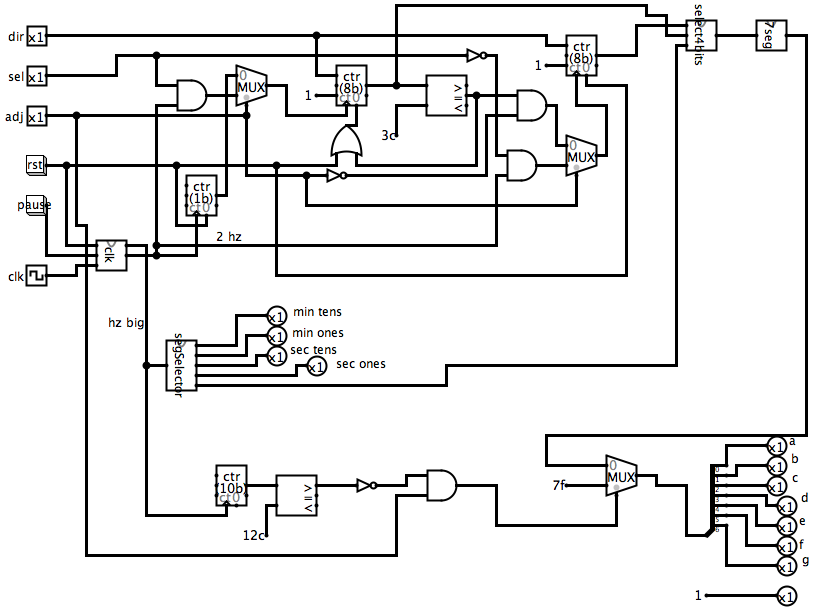
\includegraphics[width=1\textwidth]{main.png} 
		\caption{Digital Logic Design}
	\end{center}
\end{figure}

The above figure depicts the overall logic design of our circuit. The outputs a-g and p represent the segments to be lit up on the 7-segment display. The output min tens, min ones, sec tens, and sec ones represent which of the four screens on the 7-segment display should be activated where 0 corresponds with being lit up. In this figure, I black-boxed 4 components: clk, segSelector, select4bits, and 7seg. Diagrams for these components are shown below. This module uses two counters to count the minutes and seconds. The minutes are triggered by the seconds reaching 60, at which point the seconds counter overflows back to 0. Another counter is used to simulate a 1 Hz clock by controlling it with a 2 Hz clock. When reset is triggered, seconds and minutes are reset to 0, and the clock is reset back to zero as well. Pause is fed into the clock module, which will pause the 2 hz clock so that the seconds and minutes will never increment. The counter at the bottom of the screen is used to make the display blink when adjust is on. It will make the display be all 1's (all off) during a certian count, and then it will make the screen display regularly otherwise. Adjust being on will also make the seconds or minutes (depending on the select bit) increment with the 2 Hz clock. This is implemented by feeding the 1 Hz and 2 Hz clock into multiplexers, with adjust as the select bit. The output of these multiplexers goes to the clock of the counter.

\begin{figure}[H]
	\begin{center}
		%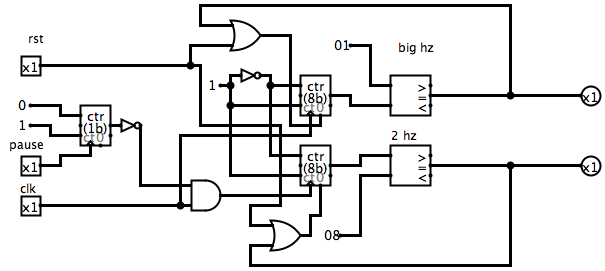
\includegraphics[width=1\textwidth]{clk.png} 
		\caption{Clock module logic}
	\end{center}
\end{figure}

This clock module takes in reset, pause, and the 100 MHz clock as input and uses counters to output a 2 Hz clock and another clock that is much faster. The counter resets after it counts to its desired Hz. A comparator is used to tell when the counter has reached a certian number. When reset is triggered, the counter will be reset to zero, and when pause is triggered, the counter will not increase.

\begin{figure}[H]
	\begin{center}
		%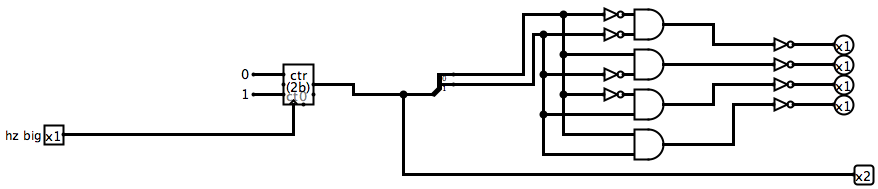
\includegraphics[width=1\textwidth]{segSelector.png} 
		\caption{Segment selector logic}
	\end{center}
\end{figure}

This module selects which of the four screens should display a digit on the seven segment display. It takes in the faster clock as an input. The output includes four bits, each bit corresponding to a screen where a 0 signifies that the screen should be lit up. The module also outputs a 2 bit integer which represents the screen number (0-3) that is being lit up this clock cycle. This module uses a counter that counts 0-3 and resets to 0 when it gets to 3 to determine which screen to light up.

\begin{figure}[H]
	\begin{center}
		%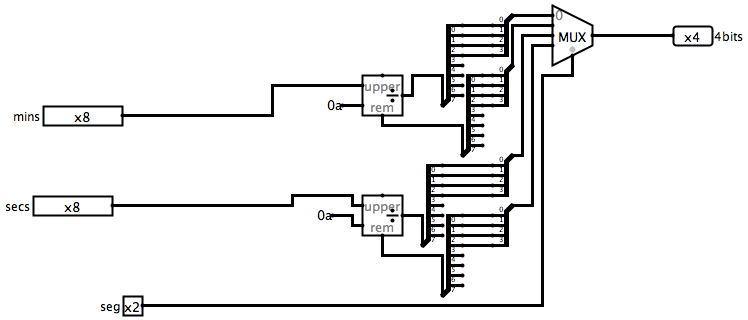
\includegraphics[width=1\textwidth]{select4bits.png} 
		\caption{Integer to display logic}
	\end{center}
\end{figure}

This module takes in as input two 8 bit integers representing the number of seconds and the number of minutes. These are fed into a divider, which essentially gets the ones and tens digits of these numbers. So we feed in the ones and tens digits of the seconds and minutes into the multiplexer, with the two bit screen integer from the segment selector module as the selector. The output is not a 4 bit integer which represents a number 0-9 to be represented on the 7 segment display. 

\begin{figure}[H]
	\begin{center}
		%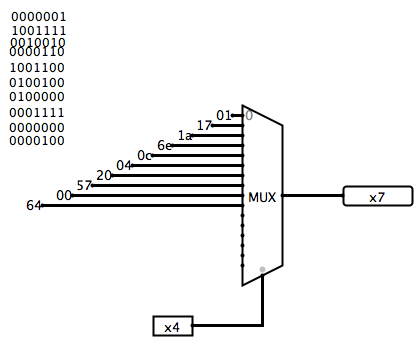
\includegraphics[width=1\textwidth]{7seg.png} 
		\caption{Four bit integer to 7 segment logic}
	\end{center}
\end{figure}

This module takes in a 4 bit integer and outputs the corresponding 7 segment display bits. The 4 bit integer is used as a selector and the left side of the multiplexer takes in 10 constants. These constants correspond to the 10 bit streams on the top of the circuit diagram. The rest are don't cares because the multiplexor should not ever get a selector that is not in the range of 0-9.

%----------------------------------------------------------------------------------------
%	SECTION 3
%----------------------------------------------------------------------------------------

\section*{Simulation}

%Simulation documentation (10%). Document all the simulation efforts (what
%requirements are tested and what the test cases are), document bugs found
%during simulation, and provide simulation waveforms. Include all simulation
%testbench code source files.
Unlike previous labs, we did not implement a test bench simulation file.  Initially, we attempted to create one for our various modules, but after having issues with uninitialized values, we chose to simply move on from this and test it via the actual FPGA board.  As to why the test bench file failed, we suspect it had to do with the clk input.  Regardless of the issue, we tested our stopwatch modules through the board using the synthesize and compilation process similar to Lab 1 (more specifically the: Synthesize->Translate->Map->Generate-> iMPACT).  
	In order to simulate our modules this way, we grabbed and modified the .ucf file from Lab 1, which allowed us to map the inputs and outputs to the correct buttons, lights, and switches on the board.  Once our code was syntactically correct, we generated a .bit file in order to implement and run the program we wrote on the board. 
	The process was generally very straightforward and smooth.  Our initial simulation effort was to light up the seven segment display; this helped us understand which values mapped to which lights allowing us to write a priority encoder of the different numbers to display.  Once that was working, we implemented clocks had to find the right speed with our fastest clock to emulate all of the 4-digits displaying at the same time without any blinking. After we had the clocks clearly working (with regards to actual, real time), we actually sped them up for testing purposes, so instead of waiting a minute to see if our minutes were decrementing correctly, we only had to wait about 30 seconds. 
	With the general clocks working, our next simulations were all based off of the various switches.  The process was relatively the same for ADJ, SEL, DIR.  ADJ worked well initially, but it had two bugs: there was no blinking of the display, which we simply forgot to code, and adjusting the seconds would eventually lead to the minutes changing as well (as in if ADJ was increasing seconds, once it hit 59, it would increment minutes by 1) .  These were both easy cases to fix, and once ADJ was working, SEL worked perfectly without any bugs to be found.  Similarly, DIR worked without any bugs on our first implementation.  We later had to test these together with the buttons, to make sure none of them lost functionality.
	After the switches were all working, we began testing the buttons.  We mapped the reset button to the center top button, and on testing it, it worked without any problems.  However, the Pause Button caused the most issues with simulation.  The debouncer was fidgety causing the pause to be inconsistent.  We tested multiple values for our debouncer, which was easily the most tedious portion of simulation, as reimplementing/compiling took nearly 4-5 minutes each time we adjusted these values.  Finally, after finding a value that we found consistent, we pressed the pause button over 300 times with a ~96\% success rate.  
	Overall, the simulation process was relatively easily, but a bit tedious.  Having to wait 4-5 minutes as well as trying to check all of the various cases to make sure things worked together was very time consuming, not to mention all of the different potential combinations was troublesome to even consider.  However, these cases, including: pausing and unpausing to make sure it stopped in between the second, reset not causing arbitrary delays, and using the different buttons with various switch combinations, all worked as the assignment specified.  


\section*{Conclusion}


%Conclusion (5%). Summary of the design. Difficulties you encountered, and
%how you dealt with them. General suggestions for improving the lab, if any.

Overall, our stopwatch design worked well, but the code itself was rather messy.  This could have been averted had we used more modules, but by the time things started getting more intricate, it wouldn't have made sense to go back and clean up what was already working.  The actual difficulties we encountered were almost all due to the debouncer for the pause button as well as the time it took to simply implement our program on the FPGA board.  Regarding the pause button: sometimes, it would be incredibly accurate, only to become less accurate the next day.  Part of this may have been which board we used (as the board the TA provided worked far more consistently), but overall, with consistent, solid presses, the pause button worked well.  
	Realistically, the only way to deal with the problem of long compilation times was by being patient.  Early on when there were still several things to implement, we would synthesize and compile, and while this was going on, we would start writing code for the next stopwatch feature.  All in all, this lab doesn't need much adjustment, however, being clearer on the various corner cases in the spec would have been helpful. 

%----------------------------------------------------------------------------------------
%	BIBLIOGRAPHY
%----------------------------------------------------------------------------------------

%\bibliographystyle{apalike}

%\bibliography{sample}

%----------------------------------------------------------------------------------------


\end{document}